\chapter{Experimental Setup and Results}
\label{ch:experimental-results}

%\begin{itemize}
%	\item Introduction about application and high-level explanation of what we'll be looking into
%\end{itemize}

In \autoref{ch:methodology} a framework was proposed for finding an optimal \acrshort{acr:mdp} for planning problems that involve uncertainty given a dataset describing the dynamics of the system under consideration.
The framework aims to achieve this by posing the adjustment of the parameters of model learning algorithms as an optimization task in which the yielded performance is to be maximized.
The domain of mobile robot navigation, where the problem statement is to navigate a robot between locations as fast as possible, was identified as a potentially suitable application.
This chapter discusses the experiments that were conducted to evaluate the framework for this application and the results that were obtained accordingly.
First of all, \autoref{sec:setup} elaborates upon the setup for the experiments, discussing the relevant details on the implementation of the framework for this application and the software and other resources used.
Subsequently, \autoref{sec:scenarios} discusses the different configurations that shall be used to test the framework.
This for instance involves various combinations of learning algorithms and different settings of the discount factor $\gamma$ and weight parameter $\beta$ on different environments.
In, \autoref{sec:results} the results obtained for these different configurations are presented, inspected and compared to one another, after which the most notable conclusions that can be drawn are discussed.

\section{Setup}
\label{sec:setup}

For our experiments we made an implementation of the framework in the form of a module that can be used to learn an optimal \acrshort{acr:mdp} for the navigation of a mobile robot.
This implementation allows the control of a mobile robot in simulations by an \acrshort{acr:mdp} and a corresponding policy.
The model values assessed from these simulations are used to find a globally maximizing parameter-settings of the learning algorithm used.
In this section we will describe the implementation in detail and how it is used in our experiments to find performance-maximizing \acrshortpl{acr:mdp} for a mobile robot in an office environment.

\subsection{Software}
\label{sec:software}

In this section we discuss the software that is used in the implementation of our optimization module. 
An overview of the main packages used for this implementation is presented in \autoref{tab:software-packages}.
In the remainder of this section, we briefly explain for what part of the implementation each of these packages are used, and support the choices made where necessary.

\begin{table}[pt]
\caption{Software packages used for the implementation of the model learning framework for mobile robot navigation.}
\label{tab:software-packages}\centering
\begin{tabular}{lll}
	\hline%
	\textbf{Package Name} & \textbf{Version} & \textbf{Purpose} \\
	\hline
	\texttt{bayesian-optimization} & 0.4.0 & Bayesian optimization \\
	\texttt{matplotlib} & 1.3.1 & Plotting and visualizing robot actions \\
	\texttt{numpy} & 1.12.1 & Array data storage and manipulation\\ 
	\texttt{pymdptoolbox} & 4.0\_b3 & \acrshort{acr:mdp} planning algorithms \\
	\texttt{ros-indigo-strands-desktop} & 0.0.14 & Simulation software and environments\\
	\texttt{scikit-learn} & 0.18.1 & Machine learning algorithms \\ \hline
\end{tabular}
\end{table}

\subsubsection{Python Libraries}
\label{sec:software-packages}
The module has been implemented in Python 2.7, due to its easily usable libraries for machine learning and plotting and other widely available packages, but also because of its convenient capability of interacting with the simulation software used.

For \acrshort{acr:mdp} planning, the \texttt{pymdptoolbox} library \cite{cordwellpymdptoolbox}, is used, which implements various planning algorithms for discrete-time \acrshortpl{acr:mdp}. 
To solve for optimal policies in learned \acrshortpl{acr:mdp} we rely on this library and apply the \acrshort{acr:vi} algorithm with a discount factor of $\gamma = 0.95$.
%Given the matrices with the transition probabilities and rewards and algorithm-parameters like a discount factor $\gamma$, these planning algorithms can produce a policy vector and a corresponding value function.

For the machine learning algorithms used, we employ the \texttt{scikit-learn} library. These algorithms include $k$-Means clustering and \acrfull{acr:gmm}.

For \acrlong{acr:bo} the \texttt{bayesian-optimization} library \cite{nogueirabayesianoptimization} has been employed. This library offers an implementation of the \acrshort{acr:bo} procedure based on a \acrshort{acr:gp} prior including the implementation of the most-used acquisition functions such as \acrshort{acr:mpi}, \acrshort{acr:mei} and \acrshort{acr:gp-ucb}.

The further Python packages used, have been listed in \autoref{tab:software-packages} and include \texttt{numpy} for the manipulation of arrays and matrices used in the implementation and \texttt{matplotlib} for creating the various plots shown in this chapter.

\subsubsection{Simulator and Mobile Robot}
\label{sec:simulator}

% Make figure with two subfigures
\begin{figure}[t]
\centering
\begin{minipage}{0.4\textwidth}
	\centering
	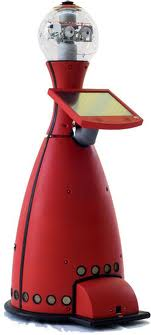
\includegraphics[width=0.3\linewidth]{scitosa5_1_model}
	\captionof{figure}{The SCITOS-A5, mobile service robot by Metralabs GmbH \cite{Metralabs}}
	\label{fig:scitosa5}
\end{minipage}
\qquad
\begin{minipage}{0.4\textwidth}
	\centering
	\vspace{23pt}
	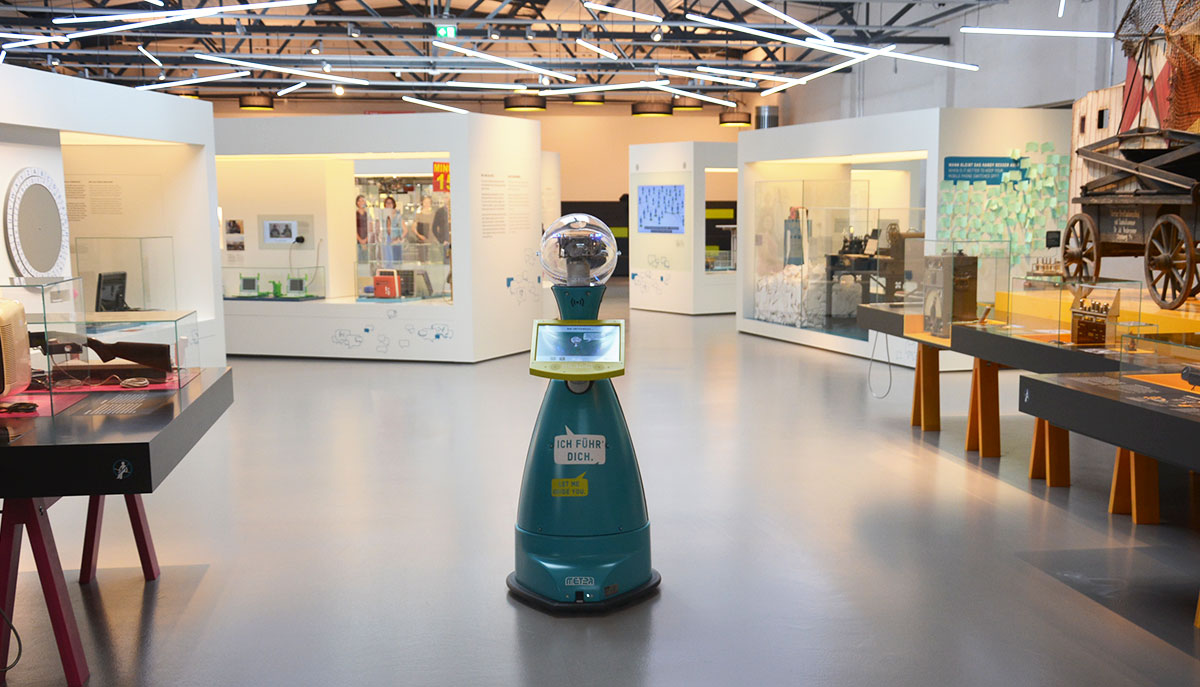
\includegraphics[width=1.1\linewidth]{scitosa5_2_TIM}
	\vspace{-10pt}
	\captionof{figure}{The SCITOS-A5 in one of its application environments. Shown here is robot \textit{TIM}, used for leading visitors of the German Technical Museum in Berlin through the exhibits \cite{Metralabs}.}
	\label{fig:scitosa5_2}
\end{minipage}
\end{figure}

For performing simulations the \textit{MORSE} simulator \cite{morse_simpar_2012}, a generic simulator for academic robots, has been used in combination with the \textit{ROS} middleware to control the robot in the environment.
The simulations are performed with the Metralabs GmbH \textit{SCITOS-A5} \cite{Metralabs}, depicted in \autoref{fig:scitosa5}, an industry-standard mobile service robot designed specifically for interacting with humans and guiding them to products or exhibits (e.g., see \autoref{fig:scitosa5_2}).
This robot is equipped with several sensors which can be used for navigation and \acrfull{acr:hri}, such as an omni-directional camera, 24 ultrasonic sensors, a collision sensor and a SICK laser range finder \cite{gross2008shopbot}.
As described in \autoref{sec:implementation} we are particularly interested in the odometric capabilities of the robot for the implementation that has been used in our experiments.
The \texttt{strands-desktop} meta-package (developed as part of the \textit{STRANDS} project \cite{hawes2016strands}) was used to obtain all required simulation software mentioned above with ease, in which the environments used in the simulations of our experiments are contained as well.



%
%\vspace{12pt}
%\noindent\fbox{\textbf{TODO:} Not completely finished yet.}

%Software used for the implementation:
%\begin{itemize}
%	\item Programming Language: \textit{Python (2.7)} together with \texttt{scikit-learn}, \texttt{pymdptoolbox}, \texttt{bayesian-optimization} packages + explain what each of them are used for
%	\item Simulator: \textit{Morse}
%	\item Scitos-A5 robot, mobile service robot (plus \textit{short} discussion of what this robot has been used for in the real world)
%	\item Control movements of robot in simulator through \textit{ROS}
%\end{itemize}

\subsection{Datasets}
\label{sec:datasets}

\begin{table}[pt]
	\caption{Metadata about the execution traces obtained}
	\label{tab:datasets-environments}\centering
	\begin{tabular}{|l|l|l|}
	\hline
	\textbf{Environment} & \textbf{Area} & \textbf{Number of entries in dataset} \\
	\hline
	\texttt{tum\_kitchen}&               &                                       \\
	\hline
	\texttt{uol\_bl}&               &            						\\ \hline          
	\end{tabular}
\end{table}

In order to be able to learn \acrshortpl{acr:mdp} from data and establish the optimization, we should obtain a dataset that  describes the environment the robot will operate in.
This dataset should describe possible robot poses and to what other poses the execution of the possible actions may lead to, in order to properly describe the dynamics of the system.

For our implementation and the experiments that have been carried out, execution traces have been obtained by letting the robot follow a random action policy during which subsequent poses and actions are logged to a file.
This exploration is performed inside the simulator both for a relatively small environment (i.e., \texttt{tum\_kitchen}) and  large environment (i.e., \texttt{uol\_bl}) obtained from a repository of the \textit{STRANDS} project.

%Explain how the data-sets are obtained. 
%- For multiple environments - What is obtained. - How the data is obtained.

\subsection{Implementation}
\label{sec:implementation}

Details on the implementation; how the framework/routine is implemented for this application. Discuss how the following aspects are taken care of in the implementation:
\begin{itemize}
	\item Environments
	\item Exploration / Data Gathering
	\item Optimization
	\item Simulations of following policy
\end{itemize}

\subsubsection{title}

\section{Scenarios}
\label{sec:scenarios}

%Discuss the different configurations that are to be compared
%\begin{itemize}
%	\item Fixed values for $\beta$-parameter vs. gradually decreasing from $1$ to $0$
%	\item Multiple environments: small (\texttt{tum\_kitchen}); large (\texttt{uol\_bl})
%	\item Model-learning algorithms: direct clustering vs. trajectory clustering; $k$-means vs. GMM
%	\item Data-sets of different sizes
%\end{itemize}

\noindent Configurations for the basic optimization framework (only based on simulations):
\begin{itemize}
	\item Fixed value for $\beta$ (i.e., which weighs $V_\mathit{DTP}$): $0$, $0.25$ and $0.5$
	\item Acquisition functions: \acrshort{acr:gp-ucb}, \acrshort{acr:mei}
	\item GMM vs. $k$-Means (vs. trajectory clustering if time available)
	\item All available data, 75\% and 50\%
	\item Discount factor: $\gamma = 0.95$
	\item Small environment: \texttt{tum\_kitchen}; and large environment: \texttt{uol\_bl}
\end{itemize}
We need to record: number of iterations, total time passed, optimum found ($\theta_\textnormal{max}$ and $V_{\mathcal{M},\textnormal{max}}$)

\vspace{12pt}
\noindent For the cost-incremental extension we could try to observe what happens when we decrease $\beta$ gradually over time.

\vspace{12pt}
\noindent Do we want to do something with `variable resolution' as post-processing step in the experiments?

\vspace{12pt}
\noindent\fbox{\textbf{TODO:} Table to be added describing the configurations/scenarios for the experiments.}

\section{Results}
\label{sec:results}

\begin{itemize}
	\item First show results of optimization only based on simulation outcomes
	\item Then show results for the cost-incremental extension of the framework
\end{itemize}

